

\section{Renormalization Group}

In this section, we won't be able to go very deeply into the theory of the subject due to its strong mathematical nature. We will therefore only skim through the main concepts and present some numerical results, for more details see \citet{renorm_leeuwen}.

We will make use of symmetries of the physical system to improve our simulations. Usually, the more information there is available about a system, the better certain quantities can be evaluated. Close to the criticality, changes in the scale of the system can be used to better extrapolate the values to an infinite system. Close to the critical point, one of the most important properties is the invariance under conformal transformations. This also implies the invariance under changes of scale (dilation invariance). Mind that this is only true around $T_c$. To increase mathematical precision one has to define exactly what it means to \emph{change scale}. In the case of geometrical objects, the meaning is somewhat intuitive. A good example is the density in fractals, which does not change under scale transformations (remember the sand-box method in \citet{comp_phys}). However, we wikk also treat systems with different energy and spin configurations as well as different Hamiltonians. One possibility is to look at the free energy density, and its invariance. To renormalize a system means to change its scale by a factor $l$: $\tilde{L}= L/l$.  This can be done either in position, or in momentum (Fourier) space.

\subsection{Real Space Renormalization}




If the system is invariant under a certain transformation, in theory one is able to iterate this transformation infinitely often without changing the quantities in the system\footnote{[...]\emph{We can construct certain transformations on the Hamiltonian of the system for which the critical point is a fixed point. Meaning that observables do not change, no matter how many times we apply these transformations.} \citep{wilson_renorm}}. In other words, the critical point is a \emph{fixed point} for this transformation. In order to put the concept of renormalization in a mathematical framework we will give two concrete examples (renormalization of the free energy and decimation of the 1D Ising model). After that, in sec. \ref{subsec:generalization}, we will generalize the concept and present the implementation of renormalization with MC in sec \ref{subsec:MCRG}. 


\subsubsection*{Renormalization and free energy}
We consider the free energy density of a system, and require it to stays invariant under scale transformations. Since the free energy is an \emph{extensive} quantity\footnote{\emph{Extensive} quantities change with the size of the system, like the volume or the total mass of a gas. \emph{Intensive} quantities are not dependent on the system size, e.g., the energy density or the temperature.}, we have to renormalize the quantity itself to the system size. With $\tilde F$ being the renormalized free energy,
\begin{equation}
\tilde{F}\kl{\tilde{\epsilon},\tilde{H}}=l^{-d} F\kl{\epsilon, H}\text{ with }\epsilon\equiv T-T_c.
\end{equation}
We then make use of the scaling law close to the critical point:
$$
F\kl{\epsilon,H} = l^d F\kl{l^{y_T}\epsilon, l^{y_H}H}
$$
$$
\Rightarrow 
\tilde{F}\kl{\tilde{\epsilon},\tilde{H}} = l^d F\kl{l^{y_T}\epsilon, l^{y_H}H}
$$
\begin{equation}
\Rightarrow 
\tilde{\epsilon} = l^{y_T}\epsilon\text{, }\tilde{H} = l^{y_H}H.
\end{equation}

Since renormalization also affects the correlation length $\xi\propto \abs{T-T_c}^{-\nu}= \abs{\epsilon}^{-\nu}$ we can relate the critical exponent $\nu$ to $y_T$:
$$
\tilde{\epsilon}^{-\nu}\propto \tilde{\xi} = \frac{\xi}{l}
$$
$$
\Rightarrow
\tilde{\epsilon} =\frac{\epsilon}{l^{-\frac{1}{\nu}}} =l^{\frac{1}{\nu}}\epsilon=l^{y_T}\epsilon
$$
$$
\Rightarrow
y_T=\frac{1}{\nu}.
$$
The critical point is a fixed point of the transformation: at $T_c$, $\epsilon=0$, and whatever the value of the scaling factor, $\epsilon$ does not change.

\subsubsection*{Majority rule}


An easy example that can be regarded as renormalization of a spin systems is the \emph{majority rule}. One considers local groups of spins $\sigma_i$, and instead of considering them all separately taking a mean over that local group of spins: $\tilde{\sigma}_{\tilde{i}} =\text{sign}\kl{\sum_{\text{region}}\sigma_i}$ (see Fig. \ref{fig:majority_rule}). Attention must be paid on how the transformation is done. In a one dimensional lattice with up/down spins for example it would be an error to apply this transformation on an even number of spins, since the sign is then not well defined for all the possible situations. The fact that one deals with system of a finite size is also something that has to be taken into account: one can renormalize up to a certain scale, before finite size effects are visible.



\noindent
\begin{minipage}{\textwidth}
  \centering
  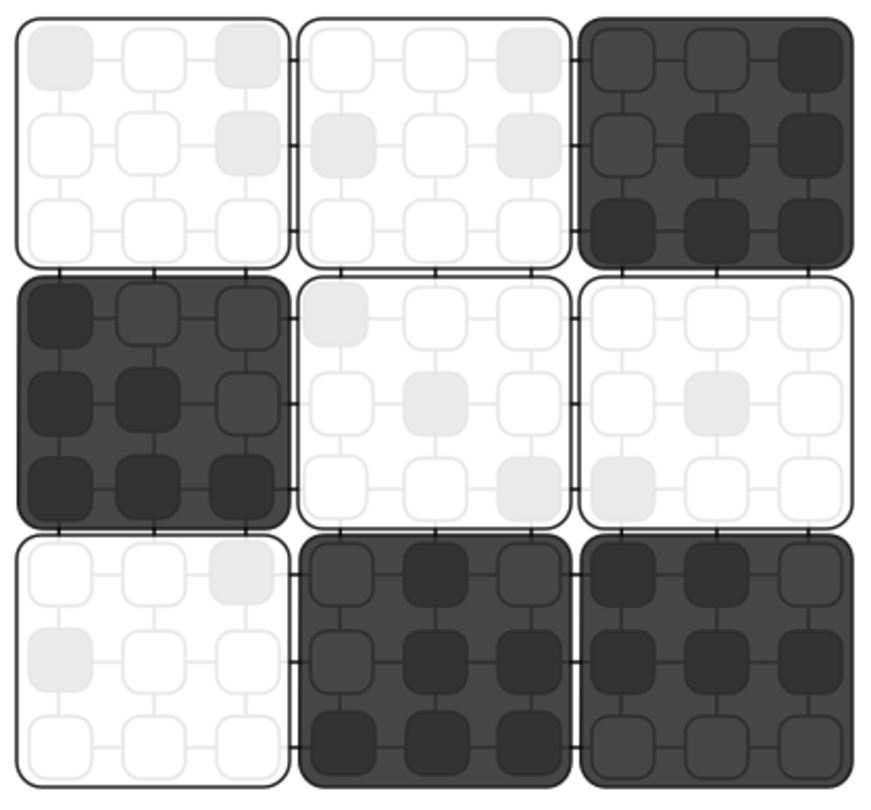
\includegraphics[width=0.5\textwidth]{pics/majority_rule}
  \captionof{figure}{Majority rule for a 2D Ising model. The spins are grouped into larger regions and averaged. If the majority of the spins is in a certain state, that region is considered as a single spin in that state.}
  \label{fig:majority_rule}
\end{minipage}




\subsubsection*{Decimation of 1D Ising Model}


Another possible rule is \emph{decimation} (see Fig. \ref{fig:decimation}). In decimation one just eliminates certain spins, generally in a regular pattern. 
\begin{figure}[h!]
  \centering
  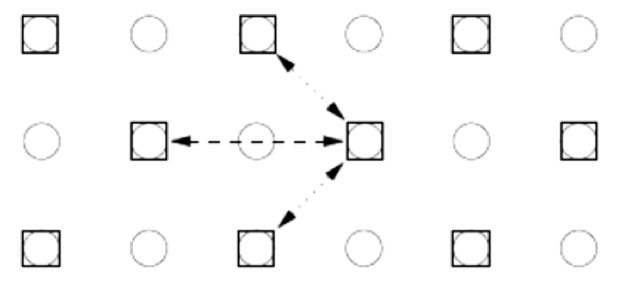
\includegraphics[height=90pt]{pics/decimation}
  \captionof{figure}{Decimation of spins: every second spin in every direction is ignored.}
  \label{fig:decimation}
\end{figure}
\vspace{0.2cm}



As already mentioned, we will consider a one dimensional Ising chain as a practical example. The spins that only interact with their nearest neighbors:

\vspace{0.2cm}

\noindent
\begin{minipage}{\textwidth}
  \centering
  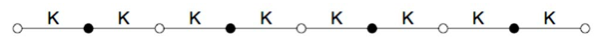
\includegraphics[height=35pt]{pics/1d_decimation}
 % \captionof{figure}{}
  \label{fig:1d_decimation}
\end{minipage}

\vspace{0.2cm}

To see explicitly what happens with the system, we calculate the partition function $Z$. We will split the partition function into two terms: one for the even sites and one for the odd sites. With $K=-\frac{J}{K_BT}$  and using

\begin{align*}
A &= \sum_{s_{2n+1}=\pm 1}{  e^  {K\kl   {  s_{2n}s_{2n+1}  + s_{2n+1} s_{2n+2}     }  } }\\
&=e^  {K\kl   {  s_{2n}+s_{2n+2}    }  }  + e^  {-K\kl   {  s_{2n}+s_{2n+2}    }  } \\
&=\text{cosh}\ekl{K\kl   {  s_{2n}+s_{2n+2}    } }
\end{align*}

we get
\begin{align*}
\mathcal{Z} &= \sum_{s_{2i}=\pm 1}{  \prod_{2i}{   \ekl{ {  
\sum_{s_{2i+1}=\pm 1}{  \prod_{2i+1}{e^  {K\kl   {  s_{2i}s_{2i+1}  + s_{2i+1} s_{2i+2}  }     }  } }  }} } }  \\
&=\sum_{s_{2i}=\pm 1}{  \prod_{2i}{  \mkl{2 \text{cosh}\ekl{K\kl{s_{2i}+s_{2i+2}}}} } }  \\
&=\sum_{s_{2i}=\pm 1}{  \prod_{2i}{  z\kl{K} e^{K' s_{2i}s_{2i+2} } } }  \\
&=\ekl{z\kl{K}}^{\frac{N}{2}}\sum_{s_{2i}=\pm 1}{  \prod_{2i}{   e^{K' s_{2i}s_{2i+2} } } }  
\end{align*}
There are only two possible states, and we can compute $z\kl{K}e^{K's_{2i}s_{2i+2}}= 2\text{cosh}\ekl{K\kl{ s_{2i}+s_{2i+2} }} $ explicitly:

\begin{equation}
z\kl{K}e^{K's_{2i}s_{2i+2}} =\begin{cases}
  2\text{cosh}\ekl{2K}  & \text{for }s_{2i}=s_{2i+2}\\
  2  & \text{for }s_{2i}=-s_{2i+2}
\end{cases}
\label{eq:condition_renorm}
\end{equation}
By dividing and multiplying the two cases we get
$$
e^{2K'} =  \text{cosh}\ekl{2K}  \text{ and } z^2\kl{K} =  4\text{cosh}\ekl{2K} 
$$
$$
\Rightarrow  K' =  \frac{1}{2}\text{ln}\kl{   \text{cosh}\ekl{2K}   }. 
$$
We have now obtained a rule after which the coupling constant $K$ (which contains the temperature and the spin coupling constant $J$) changes under scaling. In summary, we:
\begin{itemize}
\item chose the scaling rule (decimation).
\item imposed the free energy to be constant
\item computed the consequences on the coupling constant $J$
\end{itemize}



 Generally, when renormalizing a system, there are two steps that one has to undertake:
\begin{itemize}
\item Decide which scale to change (e.g., the length of the system, the spins, etc.).
\item Evaluate the consequences for the system (e.g., for the Hamiltonian, the free energy, etc.).
\end{itemize}




\subsection{Generalization}
\label{subsec:generalization}

In the above example it was possible to fulfill the condition of constant free energy with just one coupling constant. Luckily, the transformation rule for the coupling constant $K$ was enough to fulfill all the conditions expressed by eq. \eqref{eq:condition_renorm}. Generally this is not the case, and more coupling constants (e.g., next nearest neighbors) are needed to close the system of equations. We therefore have to construct a renormalized Hamiltonian made up of renormalized coupling constants which generally contain many possible interactions:


\begin{equation}
\tilde{H} = \sum_{\alpha=1}^M{\tilde{K_{\alpha}} \tilde{O}_{\alpha}} 
\text{ with }
\tilde{O}_{\alpha} =  \sum_{i}{\prod_{k\in \epsilon_\alpha}{\tilde{\sigma}_{i+k}}} 
\end{equation}
and with the renormalization rules
$$
\tilde{K}_{\alpha}\kl{K_1,...,K_M},  \text{ with } \alpha \in \mkl{1,...,M}.
$$
Note that using only $M$ interaction terms  instead of an infinite number is a truncation, and in fact a systematic error. The accuracy of this method will depend on the number of iterations that we want to take into account. At $T_c$ we have a fixed point: $\tilde{K}_{\alpha}\kl{K_1^*,...,K_M^*}=K^*_\alpha$. A first ansatz to solve this problem is the linearization of the transformation. We do this calculating the Jacobian $T_{\alpha,\beta} = \pder{\tilde{K}_\alpha}{K_\beta}$:

\begin{equation}
 \tilde{K}_\alpha - K_\alpha^* = \sum_\beta { \left .T_{\alpha, \beta}\right|_{K^*}\kl{K_\beta - K_\beta^*}}
 \label{eq:lin_trafo}
\end{equation}


\vspace{0.1cm}
\noindent
\begin{minipage}{\textwidth}
\begin{minipage}{.48\textwidth}
 We can now construct a flow chart of the coupling constant and obtain values for $\tilde{K}$ for each vector $K=\kl{K_1,...,K_M}$. At $T_c$ (where $K=K^*$), we will have a fix point. Fig. \ref{fig:renorm_flow} shows a flow diagram of a renormalization group transformation. It can already be seen that the flow is stable in some directions (the ones in which the system tends to the fixed point) and unstable in others (the ones that lead the system to go away from the fixed point). 
 \end{minipage}\hfill
\begin{minipage}{.48\textwidth}
  \centering
  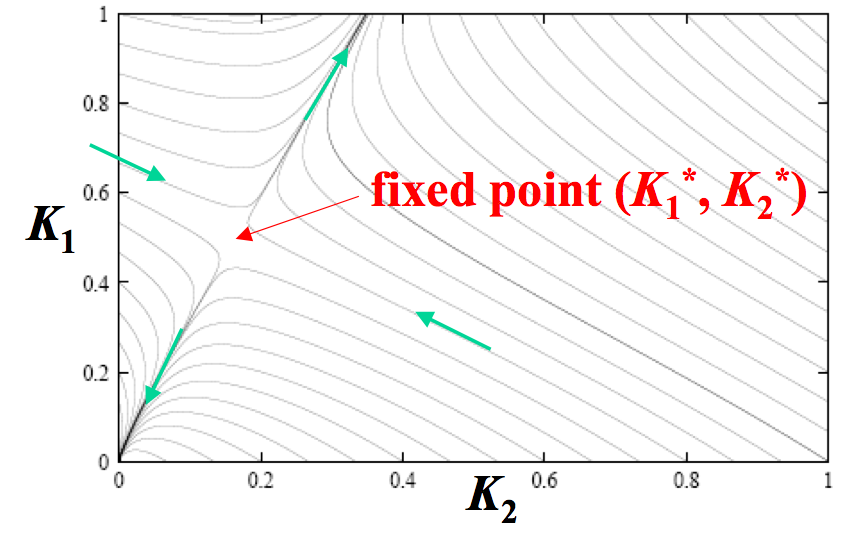
\includegraphics[height=160pt]{pics/renorm_flow}
  \captionof{figure}{Flow diagram of a renormalization transformation.}
  \label{fig:renorm_flow}
\end{minipage}
\end{minipage}

\vspace{0.2cm}


To analyze the behavior of the system close to criticality, we will consider the eigenvalues $\lambda_1,...,\lambda_M$ and the eigenvectors $\phi_1,...,\phi_M$ of the linearized transformation \ref{eq:lin_trafo}. From linear algebra we know that $\tilde{\phi_\alpha}=\lambda_\alpha\phi_\alpha$. Clearly, if $\lambda_\alpha>1$ we have an unstable situation (the distance from $\vec{K}*$ increases at every iteration of the transformation). The biggest eigenvalue will be the dominating one (which is the temperature exponent in the Ising model). We can identify the scaling field $\tilde{\epsilon}=l^{y_T}\epsilon$ with the eigenvector of the transformation, and the scaling factor with eigenvalue $\lambda_T = l^{y_T}$,

$$
\Rightarrow \nu = \frac{1}{y_T}=\frac{\text{ln}\ekl{l}}{\text{ln}\ekl{\lambda_T}}.
$$
This means that we can now calculate critical exponents using the scaling behavior of the system, if the scaling factor $l$ is known. 





\subsection{Monte Carlo Renormalization Group}
\label{subsec:MCRG}

The implementation of real space renormalization with Monte Carlo techniques was first proposed by  \citet{ma_renorm} and then reformulated by \citet{swendsen_renorm}. Since we are dealing with generalized Hamiltonians with a lot of interaction terms, we will calculate the thermal average using the operators $O_\alpha$.

\begin{equation}
\avkl{O_{\alpha}} =
\frac    {\sum_\alpha {O_\alpha e^{\sum_\beta {K_\beta O_\beta}} }  }   {\sum_\alpha {e^{\sum_\beta {K_\beta O_\beta}}}  } =
\pder {F}{K_\alpha}
\label{eq:op_av}
\end{equation}
where $F=\text{ln}\ekl{Z}$ is the free energy. Using the fluctuation-dissipation theorem one can also numerically calculate the response functions:
\begin{align*}
\chi_{\alpha,\beta} &\equiv \pder{\avkl{O_\alpha}}{K_\beta} = \avkl{O_\alpha O_\beta} -\avkl{O_\alpha }\avkl{ O_\beta}\\
\tilde{\chi}_{\alpha,\beta} &\equiv \pder{\avkl{\tilde{O}_\alpha}}{K_\beta} = \avkl{\tilde{O}_\alpha O_\beta} -\avkl{\tilde{O}_\alpha }\avkl{ O_\beta}
\end{align*}
Using the chain rule,  one can calculate with equation \eqref{eq:op_av} that



$$
\tilde{\chi}_{\alpha,\beta} \equiv \pder{\avkl{\tilde{O}_\alpha}}{K_\beta} =
\sum_\gamma {     \pder{\tilde{K}_\gamma}{K_\beta}    \pder{\avkl{\tilde{O}_\alpha^{\kl{n}}}}{K_\gamma}    }  =
\sum_\gamma  {   T_{\gamma, \beta}  \chi_{\alpha,\gamma}^{\kl{n+1}}  }.
$$
Thus we can obtain $T_{\gamma, \beta}$ from the correlation functions by solving a set of M coupled linear equations. We can iterate this method, in order to get systematically better values, if we are at the point $K=K^*$.

\vspace{0.1cm}
\noindent
\begin{minipage}{\textwidth}
\begin{minipage}{.98\textwidth}
  \centering
  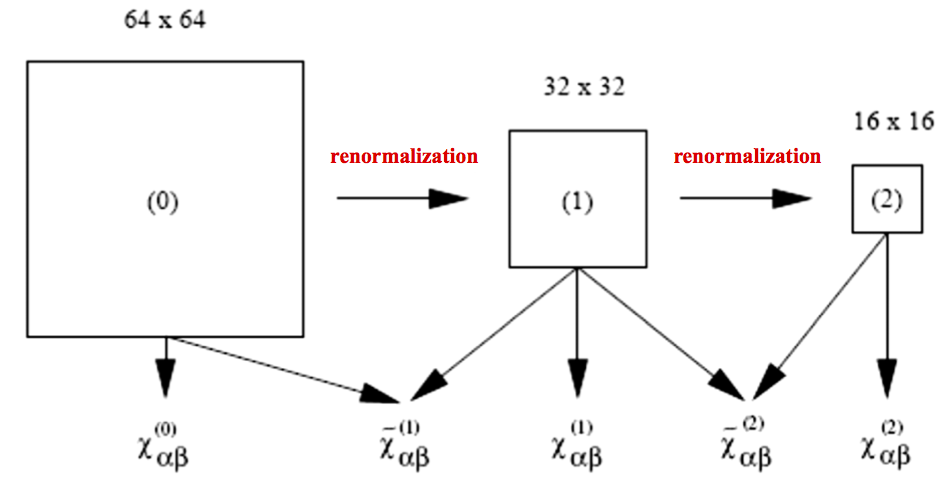
\includegraphics[height=210pt]{pics/mc_renorm}
  \captionof{figure}{Scheme of the MCRG strategy.}
  \label{fig:mc_renorm}
\end{minipage}
\end{minipage}
\vspace{0.1cm}



\vspace{0.1cm}
\noindent
\begin{minipage}{\textwidth}
\begin{minipage}{.98\textwidth}
  \centering
  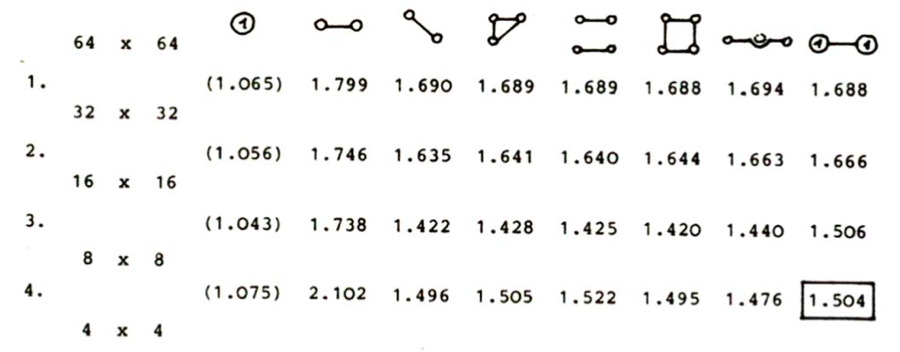
\includegraphics[height=170pt]{pics/nu4_potts}
  \captionof{figure}{$\nu$ for a 4-state Potts model in 2D. Note the convergence.}
  \label{fig:nu4_potts}
\end{minipage}
\end{minipage}
\vspace{0.1cm}



\subsubsection*{Errors in MCRG}

There are many error sources in this technique, that originate from the fact that we are using a combination of several tricks to calculate our results, of which one should be aware of:

\begin{itemize}
\item Statistical errors
\item Truncation of the Hamiltonian to the M$^{th}$ order.
\item Finite number of scaling iterations
\item Finite Size effects
\item No precise knowledge of $K^*$
\end{itemize}

















